\documentclass[a4paper,11pt]{article}
\usepackage{hyperref}
\usepackage{graphicx}
\usepackage{listings}
\usepackage{mathabx}
\usepackage{color}

\definecolor{gray}{rgb}{0.5,0.5,0.5}

\author{Maarten Inja \and Patrick de Kok}
\title{MLPR: Lab 1}

\lstset{
  language=Octave,
  basicstyle=\footnotesize,
  numbers=left,
  numberstyle=\tiny\color{gray},
  stepnumber=5,
  showspaces=false,
  showstringspaces=true
  showtabs=false,
  frame=single,
  title=\lstname,
  breaklines=true,
}
\begin{document}
\maketitle

\section*{Exercise 1}
\begin{figure}[h]
  \caption{A plot of the dataset.  The red ``$+$'' and magenta ``$\circ$'' represent the training and test data points of class A.  The blue ``$\times$'' and black ``$\convolution$'' represent the training and test data points of class B.}
  \label{plot1}
  \begin{center}
    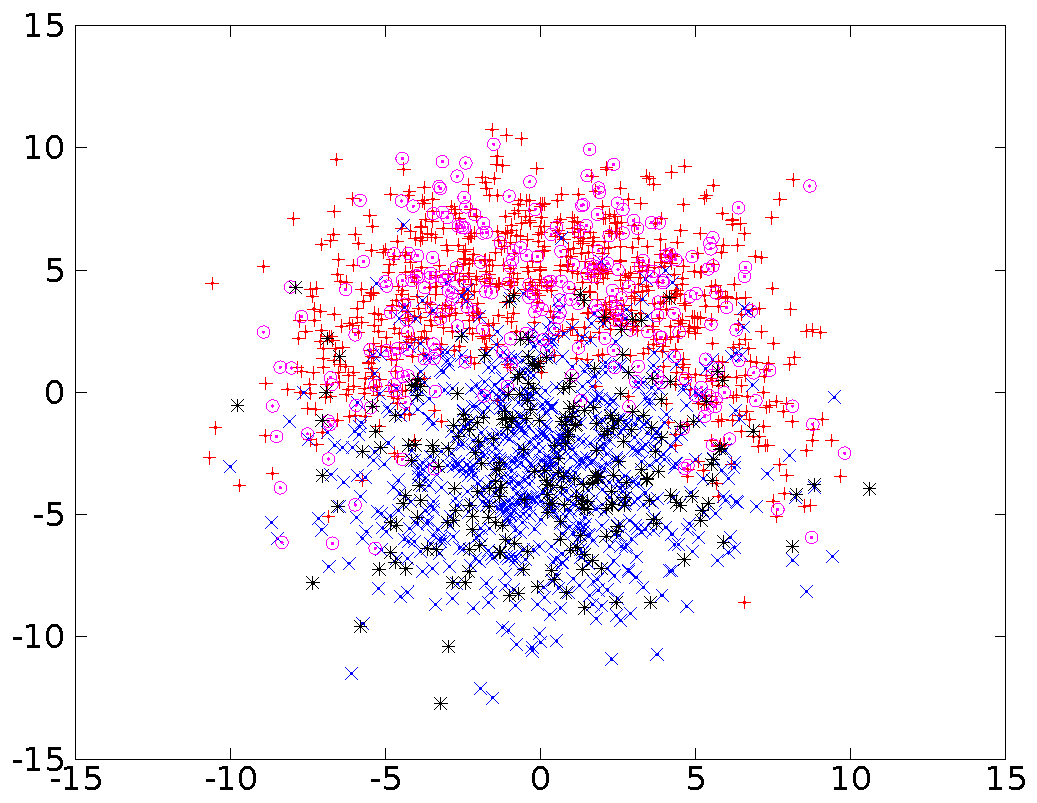
\includegraphics[width=0.6\paperwidth]{plot1}
  \end{center}
\end{figure}

Our training and test data sets are generated through the Matlab code presented in \autoref{code}.  A graphical representation is given in \autoref{plot1}.

\lstinputlisting[caption={The code which generates our data set},label=code]{lab2.m}

\section*{Exercise 2}


\section*{Exercise 3}

\end{document}
